% Figures

\begin{figure}[t]
\centering
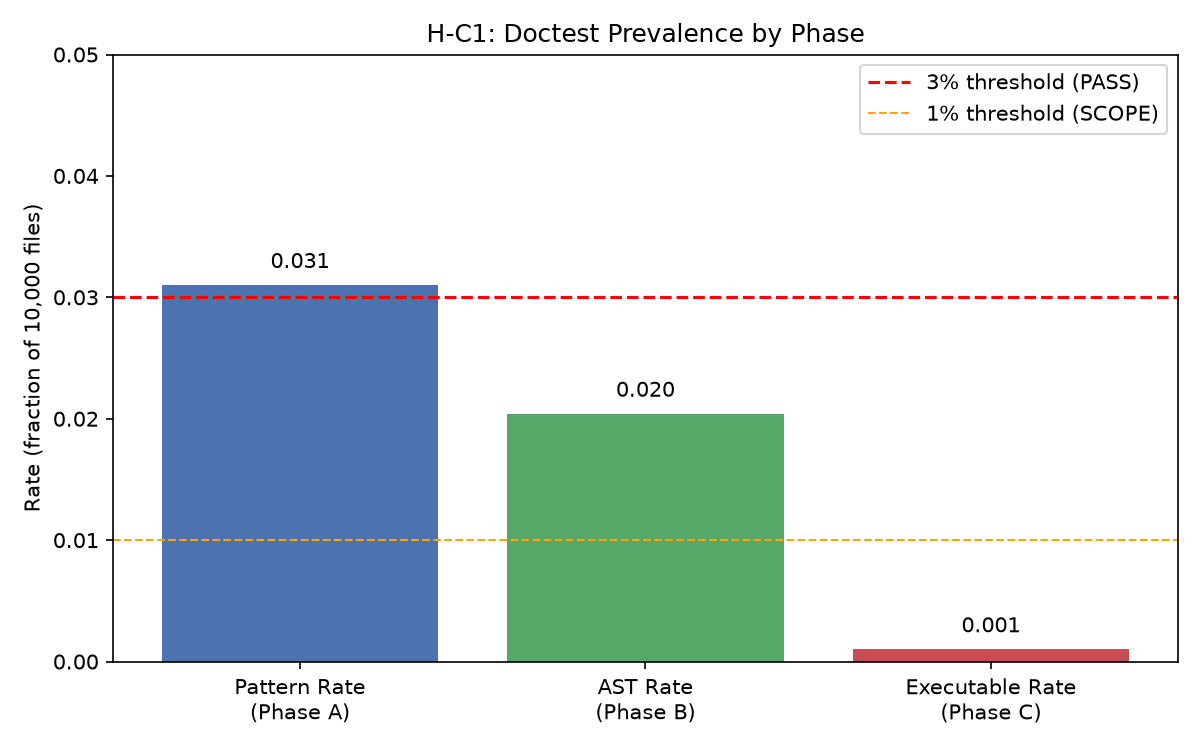
\includegraphics[width=0.85\columnwidth]{figures/gate_metrics_comparison.png}
\caption{Three-phase doctest filtering funnel: pattern prevalence (3.1\%), AST-parseable
(2.0\%), and independently-executable (0.1\%) rates across 10,000 sampled Python files.
The 3\% SHOULD\_WORK threshold (dashed line) is met by the pattern rate but not by the
executable rate, confirming PIVOT status.}
\label{fig:gate_metrics}
\end{figure}

\begin{figure}[t]
\centering
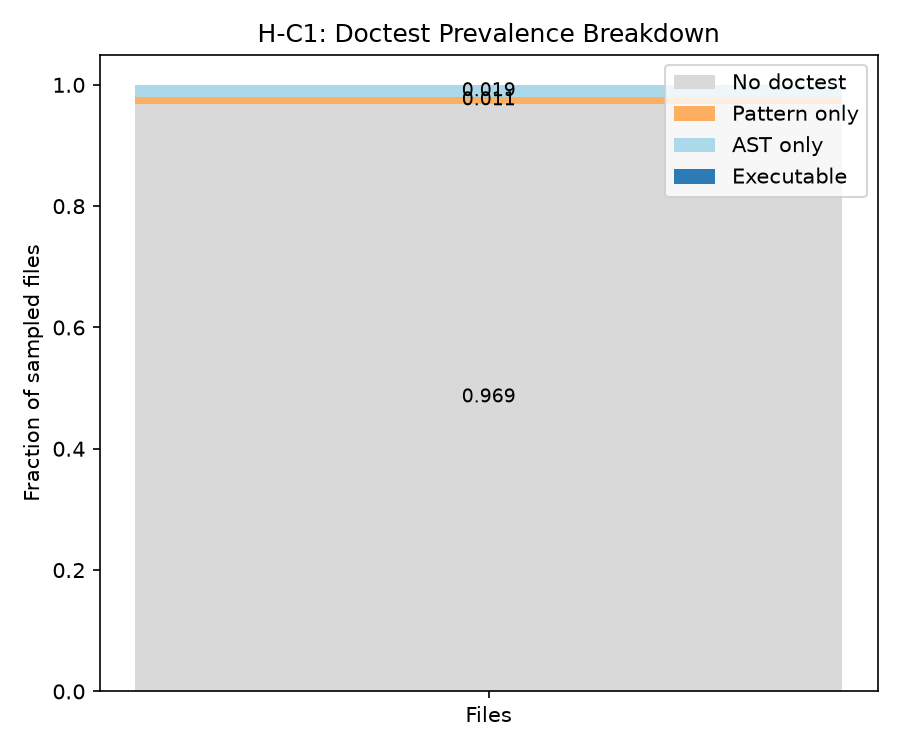
\includegraphics[width=0.85\columnwidth]{figures/prevalence_breakdown.png}
\caption{Stacked breakdown of Python files at each filtering phase, illustrating the
31$\times$ collapse from pattern prevalence to executable doctest prevalence. 96.9\% of
files contain no \texttt{>>>} patterns.}
\label{fig:prevalence}
\end{figure}

\begin{figure}[t]
\centering
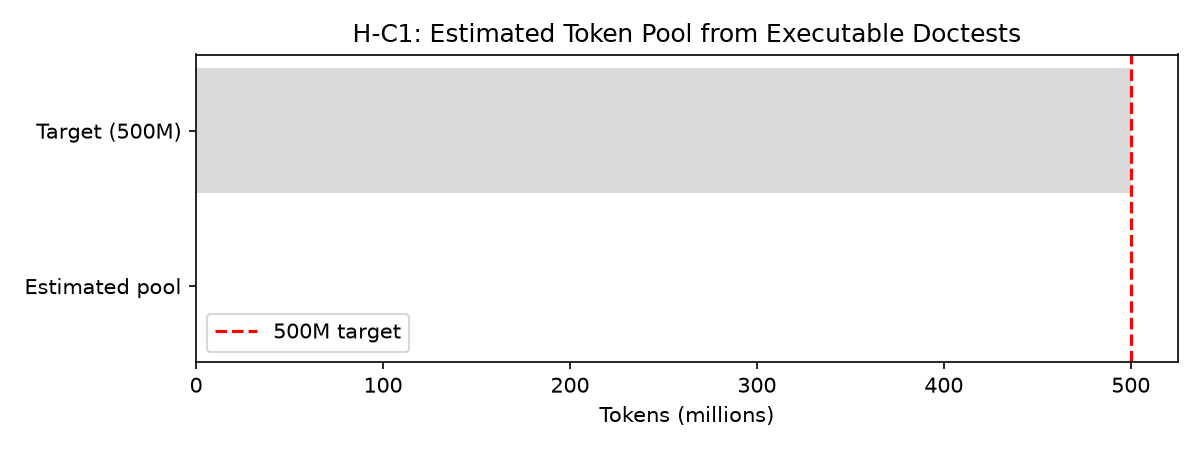
\includegraphics[width=0.85\columnwidth]{figures/token_pool_estimate.png}
\caption{Estimated token pool from executable-doctest-bearing files (0.004M tokens)
versus the 500M-token SFT budget target. The 125,000$\times$ gap establishes structural
infeasibility of the doctest-passing condition.}
\label{fig:token_pool}
\end{figure}

\begin{figure}[t]
\centering
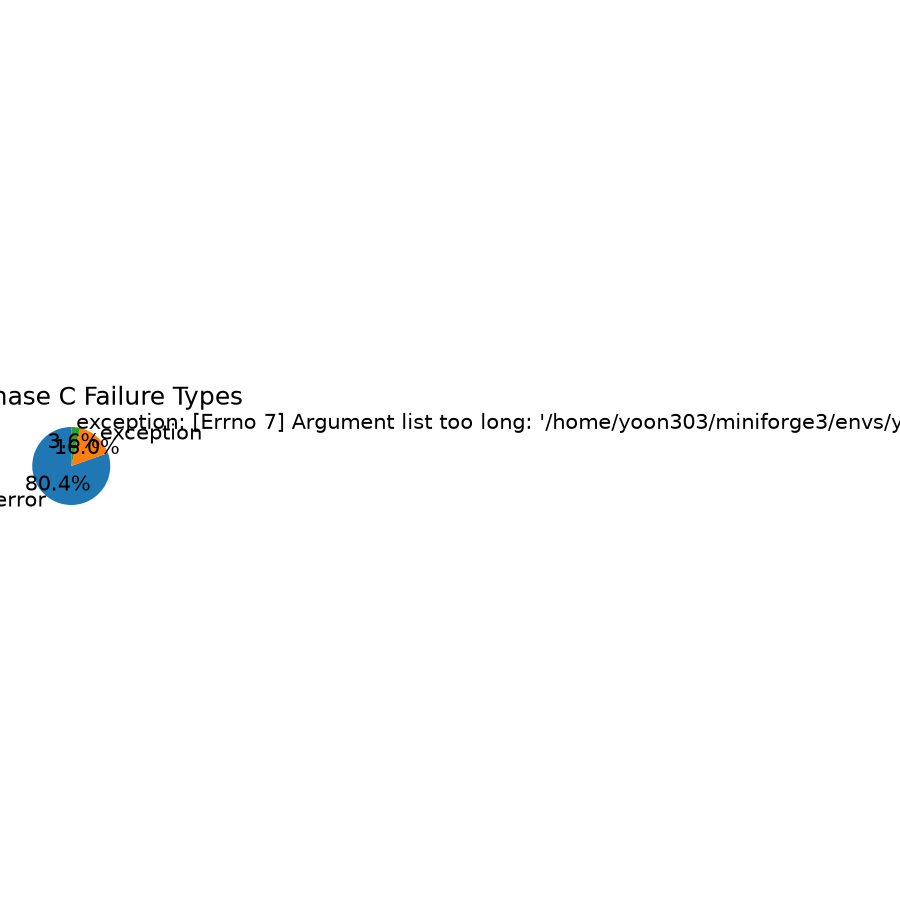
\includegraphics[width=0.85\columnwidth]{figures/error_type_distribution.png}
\caption{Distribution of Phase C (subprocess execution) failure types across 194 files
that passed Phase B. Import errors dominate, confirming third-party dependency isolation
as the primary failure mode.}
\label{fig:error_dist}
\end{figure}

\begin{figure}[t]
\centering
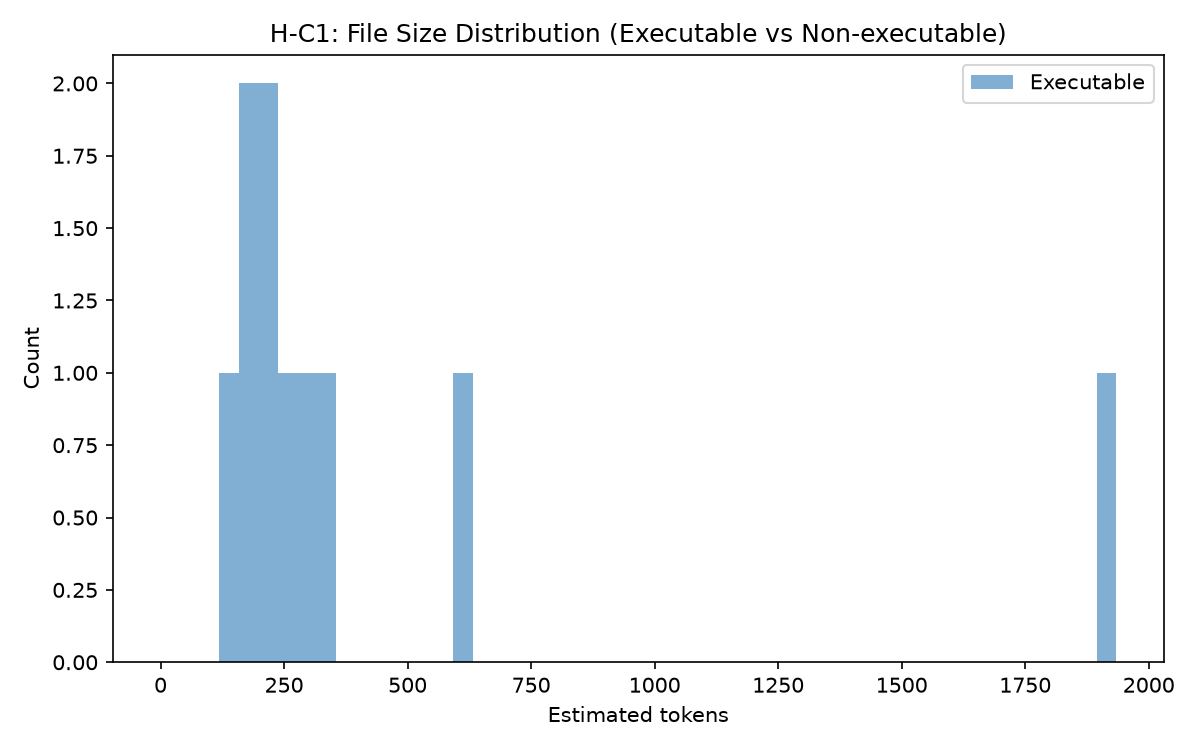
\includegraphics[width=0.85\columnwidth]{figures/file_size_distribution.png}
\caption{Token count distribution for executable-doctest-bearing files (n=10) versus
non-executable files (n=9,990), showing similar size profiles. File size is not a confound
in the feasibility finding.}
\label{fig:file_size}
\end{figure}
